% Estmal alles in einem .tex file, evtl später in mehr aufspalten ...

\section{Introduction}
Presslufthammer is an attempt at developing a prototype of the Dremel Query
System \cite{melnik2010dremel} developed by Google. Dremel is purportedly the
technology that powers the Google BigQuery \cite{bigquery} system. We will
therefore mention it in this report and also reference the BigQuery online
documentation, when talking about features of the Presslufthammer system
and comparing the functionality.

Dremel is a system that allows relational queries\footnote{BigQuery
(and Dremel) use a query language that is very similar to SQL: 
\url{https://developers.google.com/bigquery/docs/query-reference}.} to be
performed on a cluster of machines on very large datasets. The focus here
is on aggregation queries that have very small result sets compared to the
processed amounts of data and that are ``interactive'', meaning that the
results are available quick enough to work with the system interactively.

For more in-depth background information about Dremel and BigQuery you should
consult the paper or the documentation respectively. We will only highlight
the key components and difficulties in the following sections.

\subsection{Division of Work}

The Dremel systems has a very modular architecture, making it easy to share the
work. We identified to following key components (The person working on that
particular component is mentioned in parentheses):

\begin{itemize}
  \item Columnar data representation (Aljoscha)
  \item Parsing, analysis, transformation and execution of Queries (Aljoscha)
  \item Network architecture (Fabian)
  \item Utilities and stuff (Aljoscha, Fabian)
\end{itemize}

Each of these described in their own section respectively.

\subsection{Some Notes}
The Presslufthammer system is implemented in Java and makes use of several tools
and libraries to realise different features:

\begin{itemize}
  \item Maven \cite{maven} for the build system
  \item ANTLR \cite{antlr} for implementing the query parser
  \item Netty \cite{netty} for the network layer
  \item slf4j \cite{slf4j} for logging
  \item Jetty \cite{jetty} as web server for a frontend and
  \item Google guava libraries \cite{guava} because they are just plain helpful
\end{itemize}

All package names of Presslufthammer are of the form\\
\texttt{de.tuberlin.dima.presslufthammer.*},\\
but we omit the first part in the following sections for the sake of simplicity,
i.e. package \texttt{data} instead of package
\texttt{de.tuberlin.dima.pressluzfthammer.data}.


\section{Columnar Data Representation}

\section{Query Processing}

\section{Network Architecture}
  This section presents the components that comprise the network architecture
  we implemented to create the Presslufthammer system.
  All classes of the network architecture are located in the \texttt{transport}
  package and it's child packages \texttt{messages} and \texttt{util}.
  
  
  \subsection{Looking at Dremel}
    First take a look at the way the Dremel \cite{melnik2010dremel} system is
    organised.
    It consists of a multi-layered architecture including:
    \begin{itemize}
      \item A client to provide the user interface
      \item A root server to communicate with the client as well as to dispatch
        queries
      \item Multiple intermediate servers
      \item Multiple leaf servers to access the data and execute queries on it
      \item And finally a seperate storage layer holding the data
    \end{itemize}
    This is illustrated in \figref{netarch}.
    \begin{figure}[ht]
      \centering
      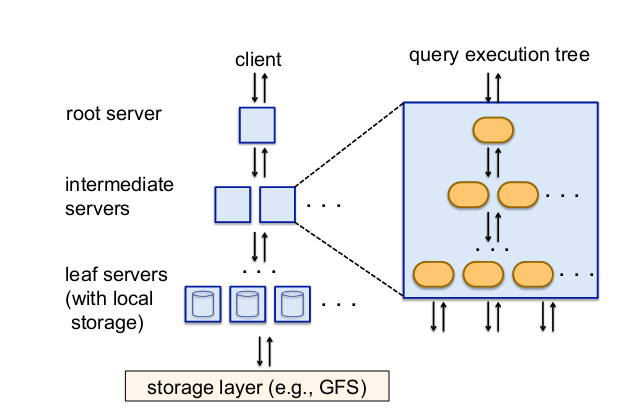
\includegraphics[width=.7\textwidth]{images/net-arch}
      \caption{The overall architecture of Dremel\cite{melnik2010dremel}}
      \label{fig:netarch}
    \end{figure}


  \subsection{Coordinator Leaf Architecture}
    For the first milestone, we implemented only a root server
    (\texttt{Coordinator}) and the leaf servers (\texttt{Leafs}),
    omitting the intermediate layer.
    This allowed us to concentrate on more basic communication features,
    such as the passing of queries and resulting data.
    \subsubsection{The Coordinator Role}
      The \texttt{Coordinator} node provides an entry point for all other nodes
      in the system.
      It is the central object used to organise the network nodes.
      Without an intermediate layer, the \texttt{Coordinator} manages all
      \texttt{Leafs} itself. It splits the queries based on available tablet
      information and distributes the parts of a query among the \texttt{Leafs}.
    
    
  \subsection{Slave Architecture}
    We then went on to implement an additional set of nodes, based on the
    idea of multi purpose nodes that can take both the role of a leaf
    and an intermediate server depending on the situation.
    These nodes are called \texttt{Slaves} and work in conjunction with the
    \texttt{SlaveCoordinator}, that replaces the aforementioned 
    \texttt{Coordinator} as root server.
    \texttt{Slaves} arrange themselves in a n-ary tree.
    The degree of the tree is configurable at instantiation
    and can differ between instances.
    This way, it is possible to create subtrees of higher or lower degree
    than the rest of the tree.


  \subsection{Client Nodes}
    The Presslufthammer system allows for multiple Client nodes to connect.
    For testing and presentation of our prototype we implemented two such
    clients.
    \begin{itemize}
      \item The first is a basic client that we use to provide command
            line access to the querying system.
            It's main purpose is the facilitating of tests.
      \item The second provides the same functionality as the first,
            but uses Jetty \cite{jetty} to provide a html based web
            interface.
            It can provide remote access to users, without the need
            to execute any client-side Java code.
    \end{itemize}
    These clients use the QueryParser to parse entered queries and obtain
    an internal representation of these.


  \subsection{Further Details}
    The network communication was realised using the Netty framework.
    All implemented nodes use the \texttt{GenericHandler} and
    \texttt{GenericPipelineFactory} classes, based on standard Netty classes,
    to send and receive messages.
    The system knows three types of network messages.
    \begin{itemize}
      \item \texttt{SimpleMessages} provide the means to transmit meta data
      \item \texttt{QueryMessages} contain the query objects used by
        Presslufthammer and
      \item \texttt{TabletMessages} encapsulate the result data of a query.
    \end{itemize}


\section{Conclusions and Further Work}
  The main difficulty in the network architecture, was the realisation of
  the intermediate layer and the parallel management of multi-part queries
  accross an execution tree.
  
  Future steps in the development of Presslufthammer could include:
  \begin{itemize}
    \item Implementation of a purely intermediate layer
    \item Implementation of a distributed storage layer (HDFS)
    \item implementation of a richer graphical user interface
    \item Improving fault tolerance
    \item Testing and Evaluation of distributed execution
    \item Performance evaluation at scale
  \end{itemize}


